We investigated three versions of the AWP design described in the last section of the previous chapter. The first type we present is based on 3D printed \ce{Al2O3}, the second type is produced using ordinary 3D printed polymers and the third type consists of SLE fused silica glass waveplates as described in the previous chapter. The results are obtained through the minimization of the two objective functions defined in the previous chapter.

% This AWP type differs from the other two in the sense that the phase shift is not caused by form birefringence, but instead by intrinsic birefringence which stems from the crystallographic orientation of the material. The second type is similar to the fused silica glass AWP in the sense that it is also based on form birefringence but the structure is 3D printed by typical of the birefringence is not from the structure but instead on the crystallographic orientation of the material. 

\section{Ceramic AWP}
In a publication by Ornik et al. it was shown that \ce{Al2O3} as a 3D printed ceramic exhibited birefringent properties. A birefringence of approximately $0.05$ was reported. This value is fairly low compared to the birefringence of sapphire which is the crystalline form of \ce{Al2O3} with a birefringence of approximately $0.32$. 

\begin{figure}[ht]
    \centering
    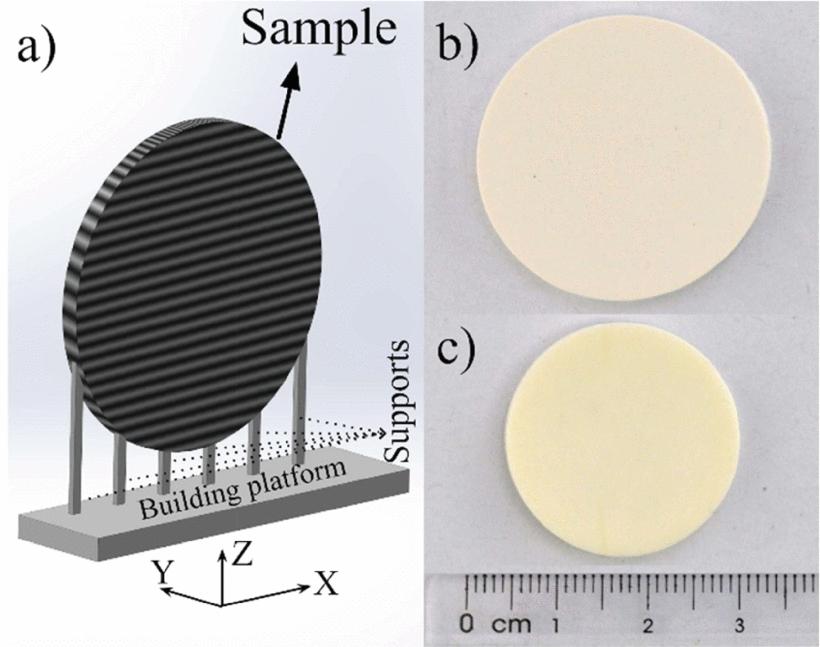
\includegraphics[scale=0.4]{images/5_chapter05/ornikabclarge.png}
    \caption{Schematic image of the a) printed sample as well as photographs of b) green and c) sintered Alumina. Source: \cite{Ornik2021}}
    \label{fig:ornik1abc}
\end{figure}
% TODO caption is copy from jan paper

It was further shown that the direction of the slow axis was parallel to the printing direction. A sketch of how the samples are printed is shown to the left in figure \ref{fig:ornik1abc}, where the arrow indicates the printing direction. The top right side shows an actual image of the green sample and the bottom right shows an image of the sample after sintering. For the sintering step the sample is slowly heated to \SI{1700}{\celsius} which causes it to shrink, in this case by around \SI{21}{\volpercent}. In total two different samples were characterized and the result of this characterization is shown in figure \ref{fig:ri_abs} \cite{Ornik2021}. The left plot shows the measured refractive index and the birefringence along the slow and fast direction for the two samples as a function of the frequency, while the right plot shows the measured absorption coefficient for the two samples and directions as a function of the frequency. We see that within the error range the birefringence of the two samples is equal. Therefore, either sample parameters works for setting up the loss function, we use the measurement result from sample 1. 

\begin{figure}[ht]
    \centering
    \includestandalone[scale=0.73]{images/5_chapter05/plots/ceramic/ri_bf}
    \caption{Left plot shows the refractive index and birefringence as a function of frequency for the two ceramic \ce{Al2O3} samples; Sample1 and Sample2. For both samples the refractive index was measured for the perpendicular slow and fast axes. Considering the error margins both samples have an equal birefringence. The right plot shows the absorption coefficient, again for the slow and fast axis of the samples. Data: \cite{Ornik2021}}
    \label{fig:ri_abs}
\end{figure}

Stacking a number of these ceramic discs or plates like the one shown in figure \ref{fig:ornik1abc} we can in theory construct an AWP similar to the TAQ by Masson. This ceramic AWP can then serve as a comparison to the TAQ and therefore also partly as a verification of the loss function at least for the $\lambda/4$ AWP type. In this case the loss functions $L_{\lambda/4}$ and $L_{\lambda/2}$ only depend on the set of angles and thicknesses. In other words the birefringence does not change at each iteration and is the same for each individual plate. An AWP of this type consisting of three ceramic discs is shown in figure \ref{fig:ceramic_stack}. Each disc has two flat sides where one is used for alignment and the other is the printing base. The alignment flat is placed keeping in mind that the slow axis is along the printing direction. In reality the discs are stacked so that ideally no air gaps in between each waveplate exists.

\begin{figure}[ht]
    \centering
    \includestandalone[scale=3.00]{images/5_chapter05/tikz_wpstack_ceramic}
    \caption{Exploded view of a ceramic AWP with $n=3$. In general each waveplate has a thickness $d_i$ and an orientation angle or azimuth $\alpha_i$. The individual plates are printed with two flat sides; one is used to align the discs and the other serves as support during the printing process. The red arrow points to the supportive base which is therefore the printing direction and hence the slow direction.}
    \label{fig:ceramic_stack}
\end{figure}


We can obtain the birefringence of quartz using the reported values in \cite{DGrischkowsky1990}. Subsequently, the Sellemeier equation allows us to interpolate the values in the available data range which is from \SIrange{0.2}{2.0}{\tera \hertz}, details can be found in the appendix section \ref{sec:sellmeier}. Using the thicknesses and angles of the TAQ given in table \ref{tab:masson_result} as well as the birefringence of quartz we can then calculate $L_{\lambda/4}(\nu)$ for the TAQ and use it for comparison. To that end we optimized $L_{\lambda/4}$ for $n=6$ in the range from \SIrange{0.25}{1.50}{\tera \hertz}. The design parameters obtained from this optimization are shown in table \ref{tab:res_cl4} (Result 1). Additionally, the terms of $L_{\lambda/4}(\nu)$ of this result as well as those for the TAQ are plotted in figure \ref{fig:loss_function_cl4} as a function of frequency. We see that the magnitude of $L_{\lambda/4}$ for these two results is similar. This indicates that $L_{\lambda/4}$ is also a suitable measure of the quality of the result similar to $L_{M}$. At around \SI{1.5}{\tera \hertz} there is a clear a cut-off for result 1 after which $L_{\lambda/4}$ increases steeply. This steep increase starts at around \SI{1.6}{\tera \hertz} for the TAQ. Defining the bandwidth as the ratio between the upper and lower frequency we get a value of  $\frac{\SI{1.5}{\tera \hertz}}{\SI{0.3}{\tera \hertz}}=5$. 

\begin{table}[ht]
    \centering
    \includestandalone[scale=1.0]{images/5_chapter05/ceramic_result_table}
    \caption{Design parameters for result 1 and 2. Both results are obtained through the optimization of $L_{\lambda/4}$ for $n=6$. In the case of result 1 the frequency range for the optimization was limited to \SIrange[range-phrase=-, range-units=single]{0.25}{1.50}{\tera \hertz} while for result 2 the range was set to \SIrange[range-phrase=-, range-units=single]{0.50}{2.25}{\tera \hertz}.}
    \label{tab:res_cl4}
\end{table}

\begin{figure}[H]
    \centering
    \includestandalone[scale=0.78]{images/5_chapter05/plots/ceramic/loss_function}
    \caption{The left subfigure shows the value of $L_{\lambda/4}$ as a function of frequency for the two results compared to the TAQ from \cite{Masson2006}. We see that in the range in which the optimization took place, the magnitude of $L_{\lambda/4}$ for the three results is fairly similar. The right subfigure shows the values of $L_M$ and $L_{\lambda/4}$ for the TAQ with respect to the frequency. The largest difference between the two is around \SI{0.5}{\tera \hertz} and \SI{0.7}{\tera \hertz}, otherwise the trend of the two functions is relatively similar.}
    \label{fig:loss_function_cl4}
\end{figure}

Similar to quartz, the birefringence of the ceramic plates is relatively low. This in turn means that for the waveplates to have an effect in the lower end of the spectrum the individual plates must be fairly thick so that we get a total thickness of around \SI{32}{\milli \meter}. Although, if we shift the frequency range of the optimization to \SIrange[range-phrase=-, range-units=single]{0.5}{2.25}{\tera \hertz} then we obtain a second result (result 2) for which the bandwidth is almost five as well $\left(\frac{\SI{2.25}{\tera \hertz}}{\SI{0.5}{\tera \hertz}}=4.5\right)$. With that the total thickness of the AWP can be reduced to \SI{26}{\milli \meter} compared to the \SI{32}{\milli \meter} of result 1. The design parameters of result 2 are given in the lower half of table \ref{tab:res_cl4} and the dotted line in the left subfigure of figure \ref{fig:loss_function_cl4} shows the individual terms of $L_{\lambda/4}$ for each frequency bound by the available material data range. The right subfigure shows a comparison between $L_M(\nu)$ and $L_{\lambda/4}(\nu)$ for the TAQ. We see that the shape of the two functions match fairly well except for the lower frequencies and especially at around \SI{0.55}{\tera \hertz} we see a large deviation. Figure \ref{fig:cl4_alpha} shows $\alpha$ for the output state given a horizontal linear polarized input as a function of the frequency for result 1 and the TAQ. Since $\alpha$ is a measure of the ellipticity of the output state it shows the difference between a circle and the shape of the output. For a circle $\alpha$ is $\arctan(1)=\SI{45}{\degree}$ which is therefore the target value. If we compare $\alpha$ for the TAQ and at the frequency \SI{0.55}{\tera \hertz} to $L_{\lambda/4}$ at the same frequency, we see that the large deviation from the optimum is correctly indicated by $L_{\lambda/4}$ while $L_M$ shows a minimum and thereby fails to recognize the deviation. We see the same situation at around \SI{0.75}{\tera \hertz}.

\begin{figure}[H]
    \centering
    \includestandalone[scale=1]{images/5_chapter05/plots/ceramic/alpha}
    \caption{$\alpha$ of the output state as a function of the frequency given a horizontal linear input for the TAQ and result 1. Ideally given a linear input the output should have an $\alpha$ of \SI{45}{\degree} independent of frequency. We see that the deviation of result 1 from the optimum is distributed more evenly on the frequency range, while for the TAQ the deviation is higher at lower frequencies.}
    \label{fig:cl4_alpha}
\end{figure}

Considering that $L_M$ and $L_{\lambda/4}$ are calculated from the same Jones matrix, which is constructed from the parameters of the TAQ and crystalline quartz, it shows that at least for some frequencies $L_{\lambda/4}$ is better at identifying deviations of the output from the optimal CP state. This could be due to the fact that the value of $L_{\lambda/4}$ is directly measures the deviation of the output from the RCP state.

To answer the question whether result 1 actually represents a zero order waveplate, we calculate the thickness required to cause a quarter wave shift at the minimum of the frequency range for a linear input state with an azimuth of \SI{45}{\degree}. In other words the thickness of a zero order quarter waveplate at at the minimum frequency which is given by equation $\ref{eq:thickness_quarter_waveplate}$. In this case the minimum frequency is \SI{0.25}{\tera \hertz} at which the birefringence is $\Delta n = 0.047$. The required thickness is therefore approximately $d_{\lambda/4}=\frac{\SI{1200}{\micro \meter}}{4\cdot0.047}=\SI{6.38}{\milli \meter}$. Comparing this value to the total thickness of result 1 we see that it is around five times lower than the total thickness and almost \SI{4}{\milli \meter} thinner than the thickest plate. If we keep in mind that a probabilistic algorithm is part of the optimization method, then this could indicate that result 1 is not the thinnest possible configuration for the given frequency range and material. On the other hand however, we have to keep in mind that $d_{\lambda/4}$ is for an angle of \SI{45}{\degree} while the six plates of result 1 are at different angles reducing the phase shift. It is therefore questionable whether we can actually directly compare $d_{\lambda/4}$ to the total thickness and if the definition of waveplate order makes sense in the context of composite waveplates. 

\begin{figure}[h]
    \centering
    \includestandalone[scale=0.8]{images/5_chapter05/plots/ceramic/convergence}
    \caption{Minimum value of $L_{\lambda/4}$ as a function of the total iteration count for the frequency range \SIrange{0.25}{1.5}{\tera \hertz} and a plate count of six. This shows that for the chosen settings the algorithm convergences rather fast.}
    \label{fig:cl4_convergence}
\end{figure}


Furthermore, if we consider two results where the total thickness of the latter is larger, then the magnitude or intensity of the corresponding output state will in general be lower compared to the output of the first result. However, $L_{\lambda/4}(\nu)$ is insensitive to isotropic changes in the absorption. So if the ellipticity and orientation of the polarization ellipses corresponding to the two results are equal for all frequencies then $L_{\lambda/4}$ will attain the same value in both cases. In other words, $L_{\lambda/4}(\nu)$ is the same for two states $\bm{\mathcal{E}}$ and $p\bm{\mathcal{E}}$, $0<p<1$ for any frequency. The intensity coefficients $p_1^2$ and $p_2^2$ for the equivalent elliptic diattenuator Jones matrix describing the result with a larger total thickness will both be scaled by $p^2$. Since in the definition of $L_{\lambda/4}$ the elements of the Jones matrix enter as a ratio, the factor $p^2$ then subsequently cancels out and both results will attain the same value of $L_{\lambda/4}$. This in turn means that there is no penalty for increasing the thicknesses other than increasing the effect of dichroism. 

To address the question whether result 1 is the global minimum or if there is a better suited one we plotted the minimum value of $\sum_{\nu}L_{\lambda/4}(\nu)$ as function of the current iteration step in figure  \ref{fig:cl4_convergence}. We see that the algorithm converges fairly fast and there are only major changes in the first 25 iterations. This indicates that finding a solution with $n=6$ which performs significantly better in the range of \SIrange{0.25}{1.50}{\tera \hertz} is unlikely using the current algorithm and loss function.

\begin{figure}[ht]
    \centering
    \includestandalone[scale=0.75]{images/5_chapter05/plots/ceramic/pe_cl4_lp}
    \caption{Polarization ellipse representation of the output states for a linear horizontal input at seven different frequencies. Left subfigure shows the output of the TAQ while the right side is for the ceramic AWP with the parameters from result 1.}
    \label{fig:cl4_pe_lp}
\end{figure}

Figure \ref{fig:cl4_pe_lp} shows the polarization ellipses of the normalized states at seven different frequencies given an initial linear horizontal input. The ellipses for the output of the TAQ is shown in the left subfigure while the right is for result 1. The arrows indicate the handedness of the polarization. We see that as expected we get LCP states in the frequency range in which the optimization took place. Outside of that range the states are significantly more elliptical. We also see a slightly better result for the intermediate frequencies compared to the lowest at \SI{0.3}{\tera \hertz}. 

\begin{figure}[ht]
    \centering
    \includestandalone[scale=0.75]{images/5_chapter05/plots/ceramic/pe_cl4_cp}
    \caption{Polarization ellipse representation of the output states for a LCP input at seven different frequencies. Left subfigure shows the output of the TAQ while the right side is for the ceramic AWP with the parameters from result 1.}
    \label{fig:cl4_pe_cp}
\end{figure}

Figure \ref{fig:cl4_pe_cp} is similar to figure \ref{fig:cl4_pe_lp} except that the input in this case is LCP. We know from the previous sections that a quarter waveplate should produce a linear polarized output for a circular polarized input. We see that this is the case for the TAQ up to at least \SI{1.50}{\tera \hertz}, after which the state increasingly deviates from the linear ellipse shape. Interestingly the ellipses of result 1 have a lower ellipticity compared to those of the TAQ, which indicates that the TAQ is better suited for turning a circular polarized input into a linear polarized output. The reason for this could be that we only consider the circularity of the output state in the loss function used to obtain result 1, while for the TAQ the resulting phase shift was directly optimized. This could therefore indicate that it is not sufficient to only consider the circularity of the output state in the loss function and a measure of the linearity should be included as well. Although, on the other hand the relatively large deviation that can be seen at \SI{1.50}{\tera \hertz} can also be recognized in the plot of the loss function in figure \ref{fig:loss_function_cl4}. Which means that the deviation is recognized by the loss function but a minimum was not found that minimizes $L_{\lambda/4}$ at this point. This could therefore further indicate that it is more difficult to minimize $L_{\lambda/4}$ compared to minimizing $L_M$.

The circular and linear polarization degrees $V_c$ and $V_l$ for a linear input state is shown in figure \ref{fig:cl4_pol_deg} as a function of frequency for result 1 and the TAQ. Subfigures (a) and (c) show the full frequency range of $V_c$ and $V_l$ respectively, while subfigures (b) and (d) show the first \SI{1.6}{\tera \hertz}. For clarity $V_c$ is offset by one in (b) so that values of $V_c$ closer to zero are in fact closer to negative one. We see that as expected $V_c$ is around $-1$ in the optimization range for both the TAQ and result 1 which indicates that the light is almost purely LCP. Interestingly, outside of the optimization frequency range the light switches to be primarily RCP. Furthermore, subfigure (b) shows that $V_c$ for result 1 varies less for frequencies below \SI{0.6}{\tera \hertz} and more for higher frequencies compared to the TAQ and varies less overall. This could be due to the difference between the refractive indices used for quartz during optimization and the values used for the calculation of $V_c$, since these deviations are fairly small. From subfigure (c) we see that the linear polarization degree increases to one and decreases again while the light switches to RCP. Subfigure (d) shows a similar trend as (b) in the sense that result 1 is closer to zero at lower frequencies compared to the TAQ. We also see that $V_l$ is not zero, the light is therefore not perfectly CP but also partly LP, which is difficult to see in the polarization ellipse representation. 

\begin{figure}[H]
\centering
\subcaptionbox{\label{fig:cl4_pol_deg_a}}
    {\hspace*{-2em}\includestandalone[width=0.45\linewidth]{images/5_chapter05/plots/ceramic/polDeg/degCirc}}
\qquad
\subcaptionbox{\label{fig:cl4_pol_deg_b}}
    {\hspace*{-2em}\includestandalone[width=0.45\linewidth]{images/5_chapter05/plots/ceramic/polDeg/degCircZoom}}

\subcaptionbox{\label{fig:cl4_pol_deg_c}}
    {\hspace*{-2em}\includestandalone[width=0.45\linewidth]{images/5_chapter05/plots/ceramic/polDeg/degLin}}
\qquad
\subcaptionbox{\label{fig:cl4_pol_deg_d}}
    {\hspace*{-2em}\includestandalone[width=0.45\linewidth]{images/5_chapter05/plots/ceramic/polDeg/degLinZoom}}
\caption{Subfigures (a) and (c) in the left column show the circular and linear polarization degrees respectively, as a function of the frequency for result 1 and the TAQ. Subfigures (b) and (d) in the right column also show the polarization degrees but for a smaller frequency range. The circular polarization degree in (b) is offset by one.}
\label{fig:cl4_pol_deg}
\end{figure}

Using the values for the absorption coefficient of quartz reported in \cite{DGrischkowsky1990} we can calculate the intensity of the light after passing through the \SI{31.45}{\milli \meter} thick TAQ. We can carry out the same calculation for the ceramic AWP designs; result 1 and the slightly thinner result 2 which have a total thickness of \SI{31.94}{\milli \meter} and \SI{26.24}{\milli \meter} respectively. The transmission as a function of frequency for these three designs is shown in figure \ref{fig:cl4_intensity}, where the right subfigure shows the range in which the optimization took place in the case of result 1. We clearly see that even though the three designs have an almost equal total thickness the insertion loss of the ceramic AWPs is several orders of magnitude higher compared to the quartz TAQ, which limits the practicality of ceramic AWPs.
A possibility to reduce the significance of this could be to decrease the bandwidth of the ceramic AWP and thereby also decrease the required total thickness. Another possibility to partly circumvent this problem could be to simply only use the lower frequency range where the absorption is lower. Additionally, the intensity of the lower frequency components is higher, at least in the case of the THz-TDS systems used in this work. Since apparently the birefringence of 3D printed \ce{Al2O3} depends on the printing process it might be possible to enhance the birefringence by modifying the printing process, which in turn means that the total thickness can be reduced. The latter is still work in progress.

\begin{figure}[ht]
    \centering
    \includestandalone[scale=0.7]{images/5_chapter05/plots/ceramic/intensity}
    \caption{Transmission as a function of frequency for result 1 and 2 compared to the quartz TAQ. In the right subfigure the frequency range is reduced to the range in which result 1 was optimized. The insertion losses of result 1 and 2 are significantly higher compared to the TAQ, which is due to the higher absorption of the ceramic plates compared to the quartz plates.}
    \label{fig:cl4_intensity}
\end{figure}

Figure \ref{fig:cl4_params} shows the two sets of parameterization angles ($\alpha$, $\delta$) and ($\psi$, $\chi$) for result 1 and the TAQ as a function of frequency. We see that the values of $\alpha$ and $\delta$ are around \SI{45}{\degree} and \SI{270}{\degree} respectively for both result 1 and the TAQ indicating LCP. Again, similar to what the polarization degree showed we see a transition to RCP outside of the optimized frequency range, where in the case of result 1 the transition is sharper. For both the TAQ and result 1 the transition happens via a decrease of $\delta$. Since the phase shift is proportional to the birefringence times the path length and increases for increasing frequency it could indicate that the birefringence is negative. Furthermore, since $\delta = \delta_y - \delta_x$ and $\delta$ decreases for frequencies above approximately \SI{1.6}{\tera \hertz}, it shows that the phase of the x-component advances faster which in turn could indicate that the fast axis is partly along the x-axis. The x-axis is defined as the axis along which the incident light is polarized. Additionally, we see a bump in $\alpha$ around \SI{1.75}{\tera \hertz}. This is likely due to the same reason that causes the sharper decrease of $\delta$ for result 1 compared to the TAQ, since $\delta$ and $\alpha$ are related via $\sin(2\chi)=\sin(2\alpha)\sin(\delta)$ and the trend of the ellipticity $\chi$ is similar in both cases. We further see that the azimuth $\psi$ changes rapidly with frequency where the vertical lines are due to the confinement of $\psi$ to the interval $\left[0, \pi\right]$. This means that if we were to use two identical AWPs of this type in series to create a $\lambda/2$ AWP it likely would not have the desired effect, since the output state is highly dependent on the azimuth of the input. As a reminder, the azimuth of the input state in all cases shown so far and for all frequencies is zero.

\begin{figure}[ht]
    \centering
    \includestandalone[scale=0.84]{images/5_chapter05/plots/ceramic/params}
    \caption{The two sets of parameterization angles ($\alpha$, $\delta$) and ($\psi$, $\chi$) a function of frequency, where the left and right subfigure shows the angles for the TAQ and result 1 respectively. The values of $\alpha$ and $\delta$ are as expected for LCP as well as after the transition to RCP for both designs. The variation of the azimuth $\psi$ makes it impossible to place two of these designs in series to form a $\lambda/2$ AWP. As expected, for LCP and RCP frequencies $\chi$ attains a value of plus or minus \SI{45}{\degree} respectively.}
    \label{fig:cl4_params}
\end{figure}



\begin{itemize}
    \item back in time we used other loss function. (described in appendix)
    \item that function gave the following design which we had printed by a third party.
    same printer as previous samples but with slightly different printing and sintering parameters and in the meantime printer had been moved to new location.
    \item (picture of the plates)
    \item we characterized them in focus/transmission setup at 3 angles 0, 90, 180 deg
    \item (plots of teralyzer eval)
    \item results showed that birefringence is almost non existing and disappears in error
\end{itemize}

% TODO fix colors and change masson in legend to TAQ
% TODO Jones paper 1941 hurwitz. unitary matrix can be represented as rotator + retarder
% TODO Add pic like fig 1 in https://doi.org/10.1364/AO.54.009758 (done)
% TODO add no, ne, bf plot of sapphire(?)
% TODO fix ylabel
% TODO what about roundness of output state? (alpha=arctan(a/b))
%\begin{itemize}
%    \item loss function. Frequency dependent loss. (done)
%    \item Circularity. Linearity. (done, res1 + masson)
%    \item Ellipses, linear and circular (r/l?) input, shown output. (done,)
%    \item alpha, azimuth, delay, ellip angle (done)
    %\item Transmission along two directions (lin -> wp -> x-pol int(out), (lin -> wp -> y-pol int(out))). Probably not? Maybe just intensity(freq) is enough
%    \item Retardance, Diattenuation
%    \item See what interface does?
%    \item Eigenstates?
%    \item compare to Result 1 -> we do shorter range because of absorption (thinner plate(s))
%    \item high abs compared to quartz (\cite{DGrischkowsky1990})
%    \item things that need mention but no plot probably: tot. pol. deg., inhomogenity, normality. Check for more.
%    \item poincare sphere (take python ss, cba to do it in latex tbh)
%\end{itemize}

\subsection{CST}
\subsection{Fabrication error}

\section{Polymer}

\section{Fused silica glass}

% Todo ref?


